\documentclass[aps,pre,twocolumn,showpacs,amsmath,amssymb]{revtex4-1}

\usepackage{float}
\usepackage{graphicx}
\usepackage{color}

\usepackage[portuguese]{babel}
\usepackage[utf8]{inputenc}
\usepackage[T1]{fontenc}
\usepackage{amssymb}
\usepackage{titlesec}

\titlespacing*{\section}{0pt}{\baselineskip}{\baselineskip}
\titlespacing*{\subsection}{0pt}{\baselineskip}{\baselineskip}

\hfuzz 1pt
\vfuzz 1pt

\setlength{\parskip}{\baselineskip}

\newcommand\restrict[1]{\raisebox{-.5ex}{$|$}_{#1}}

\begin{document}

\title{Exercício 5: Sistemas de equações (parte II)}

\author{Ernesto González 52857, Fábio Vasconcelos 52841}

\begin{abstract}

  Pretende-se resolver sistemas de equações usando o método de Newton e os métodos de Gauss-Seidel com e sem relaxação em Python e comparar com os valores obtidos no {\it Wolfram Mathematica} para o método de Gauss-Seidel, discutindo o método usado pelo mesmo.

\end{abstract}

\maketitle

\section{Metodologia}

{\bf Método de Gauss-Seidel sem relaxação:} inicialmente definem-se as matrizes A, B e X em que [A|B] é a matriz ampliada do sistema e X é a hipótese inicial de solução sobre a qual se itera. Itera-se sobre X enquanto o módulo do erro for superior à precisão ou o número de iterações ($k$) inferior a $k_{máx}$. É percorrido um ciclo de $i=1,2,...,n$ onde definem-se as variáveis $soma_{antes}$ e $soma_{depois}$. Itera-se sobre a primeira variável, percorrendo um ciclo de $j=1,2,...,i-1$ e somando $a[i][j]x[j]$ e itera-se sobre a segunda variável, percorrendo o ciclo de $j=i-1,...,n$. Por último e ainda no ciclo inicial, iguala-se $x[i]$ a $(b[i]-soma_{antes}-soma_{depois})/a[i][i]$ e o erro máximo passa a ser $(x[i]-x_{anterior}[i])/x[i]$, se for maior que o da iteração anterior.

{\bf Método de Gauss-Seidel com relaxação:} este método é semelhante ao método anterior e apenas difere no passo em que iguala-se $x[i]$ a $(b[i]-soma_{antes}-soma_{depois})/a[i][i]$, ao invés, sobre cada constante de relaxação ($\lambda$) temos $x[i]=\lambda(b[i]-soma_{antes}-soma_{depois})/a[i][i]+(1+\lambda)x[i]$.

{\bf Método de Newton:} inicialmente define-se a matriz X que é a hipótese inicial de solução sobre a qual se itera e o erro máximo inicial. O programa corre enquanto o módulo do erro for superior à precisão e o número de iterações ($k$) inferior a $k_{máx}$. Definem-se a matriz Jacobiana (J) e a matriz da função (F) e resolve-se a equação $Jd=F$. Por último, percorre-se um ciclo  de $i=1,2,...,n$ que itera sobre $x[i]$ igualando-o a $x[i]-d[i]$ e o erro máximo igualando-o a $d[i]/x[i]$ se o valor atual for maior que o da iteração anterior.

\section{Sistema de blocos e molas}

No primeiro exercício considerou-se um sistema de blocos e molas cujo equilíbrio é descrito pelo sistema de equações \ref{sistema}, em que se considera $x_i$ o deslocamento do bloco$_i$ em $mm$.
\begin{equation}
\begin{cases}
3(x_2-x_1)-2x_1=-80\\
3(x_3-x_2)-3(x_2-x_1)=0\\
3(x_4-x_3)-3(x_3-x_2)=0\\
3(x_5-x_4)-3(x_4-x_3)=60\\
-2x_5-3(x_5-x_4)=0
\end{cases}
\label{sistema}
\end{equation}
Inicialmente implementámos o método de Gauss-Seidel sem relaxação em {\it Python} e comparámos com os valores obtidos recorrendo á função {\it Solve} do {\it Wolfram Mathematica}, os mesmos encontram-se na tabela \ref{gauss_seidel_no_chill}. Para os dois métodos, verificam-se diferenças nos valores a partir da terceira casa decimal, isso deve-se a diferenças nos processos de resolução dos sitemas: o \textit{Solve} usa transformações não equivalentes para encontrar soluções de equações transcendentais, podendo dar soluções que não correspondam exactamente ao sistema apresentado..
\begin{table}[h!]
\centering
\caption{Valores das variáveis $x_i$ obtidos com o {\it Wolfram Mathematica} e implementando o método de Gauss-Seidel sem relaxação usando como critério de convergência $\varepsilon =0,0001$ e um máximo de 50 iterações. Ao correr, os valores convergiram ao fim de 39 iterações e obtivemos $x_i$ com uma precisão de 4 casas decimais.}
\label{gauss_seidel_no_chill}
\resizebox{\columnwidth}{!}{%
\begin{tabular}{|c|c|c|c|c|c|}
\hline
\textbf{Variável} & \textbf{$x_1$} & \textbf{$x_2$} & \textbf{$x_3$} & \textbf{$x_4$} & \textbf{$x_5$} \\ \hline
\textbf{Python} & 20.71569 & 7.85901 & -4.99813 & -17.85565 & -10.71339 \\ \hline
\textbf{Mathematica} & 20,71429 & 7,85714 & -5 & -17,85714 & -10,71429 \\ \hline
\end{tabular}%
}
\end{table}\\
\indent De seguida, aplicou-se o método de Gauss-Seidel com relaxação, usaram-se as constantes de relaxação $\lambda \in \{0.5,1,1.2,2\}$.
\begin{figure}[hbt!]
    \begin{center}
    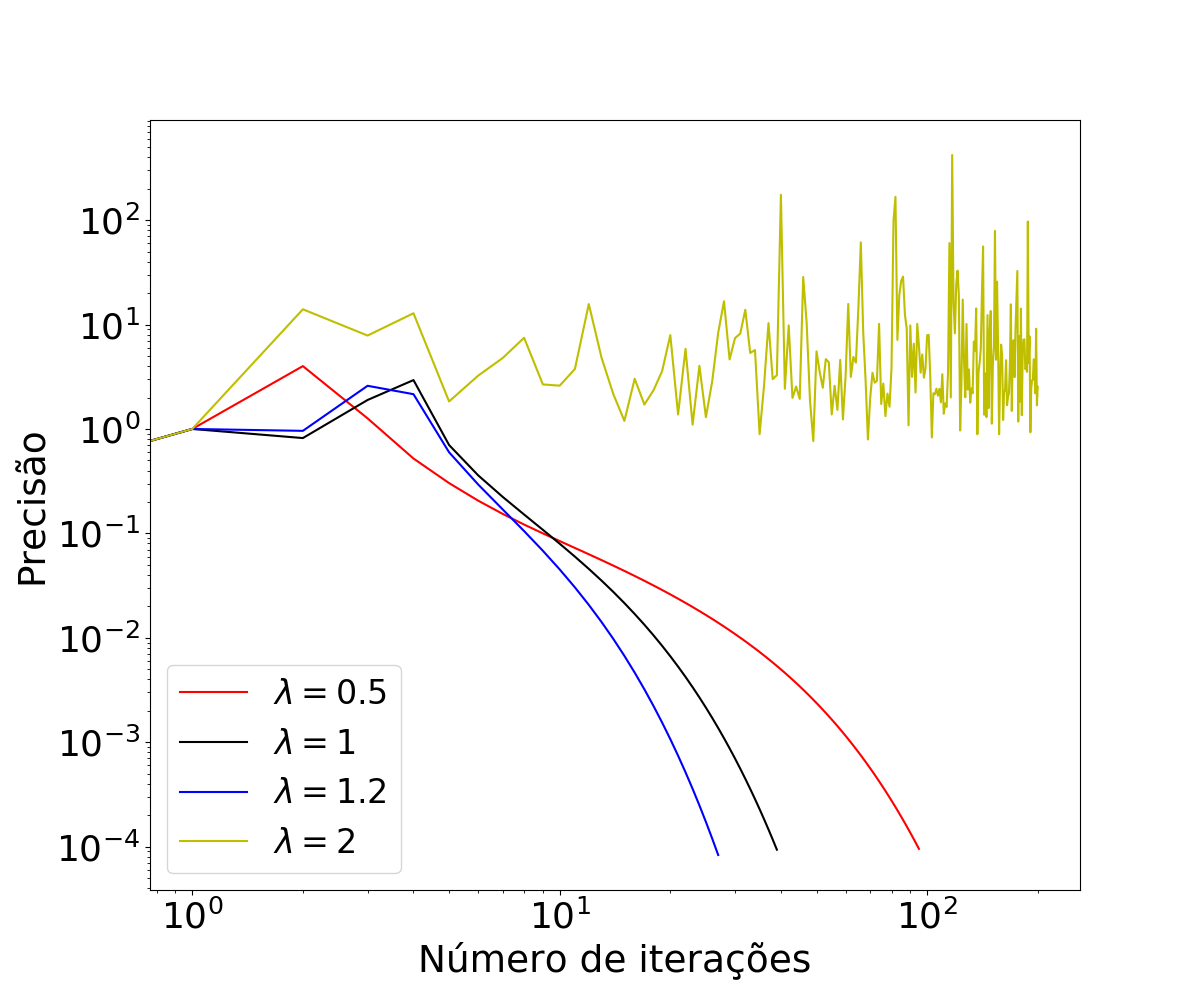
\includegraphics[width=\columnwidth]{erroPorIteracao.png}
    \caption{Gráfico da precisão em função do número de iterações para o método de Gauss-Seidel com constantes de relaxação $\lambda={0.5,1,1.2,2}$, usou-se como critério de convergência $\varepsilon =0,0001$ e um número máximo de 200 iterações. Para $\lambda =0.5$ os valores convergiram ao fim de 23 iterações, com $\lambda =1.0$ os valores convergiram ao fim de 8 iterações e para $\lambda =1.2$ convergiram após 9 iterações. Para $\lambda =1.2$ o método diverge.}% Os valores de $x_i$ para cada constante de relaxação estão na tabela \ref{erro_iter}. Quando $\lambda =2.0$, não se verificou convergência dos valores de $x_i$.}
    \end{center}
\end{figure}\\
\indent Para todos os valores de constante de relaxação os valores de $x_i$ convergiram com uma precisão da ordem de $10^{-4}$ à exceção dos valores cujo método usa uma constante igual a 2, nesse caso não se verificou convergência dos valores. A constante é demasiado grande e o que acontece é que a cada iteração o erro sobe ou desce continuamente e ocorrem erros que o método não prevê/cobre como a divisão por zero.

\section{Sistema de equações não lineares}
Considere-se, agora, o sistema não linear
\begin{equation}
  \begin{cases}
    x^2=5-y^2\\
    y+1=x^2\\
  \end{cases}
\label{sistema2}
\end{equation}

Uma forma simples de encontrar a solução deste sistema é graficamente. Para tal, definam-se as curvas parametrizadas $f_1(x)=\sqrt{5-x^2}$, $f_2(x)=-\sqrt{5-x^2}$ e $g(x)=x^2-1$. É fácil ver que os pares ordenados $(x,f_1(x)),(x,f_2(x))\in \mathbb{R}$ são as soluções de $x^2=5-y^2$ e os pares ordenados $(x,g(x))\in \mathbb{R}$ são as soluções de $y+1=x^2$. Encontram-se representados na Figura X os gráficos de $f_1$, $f_2$ e $g$.
\begin{figure}[hbt!]\vspace{-5ex}
  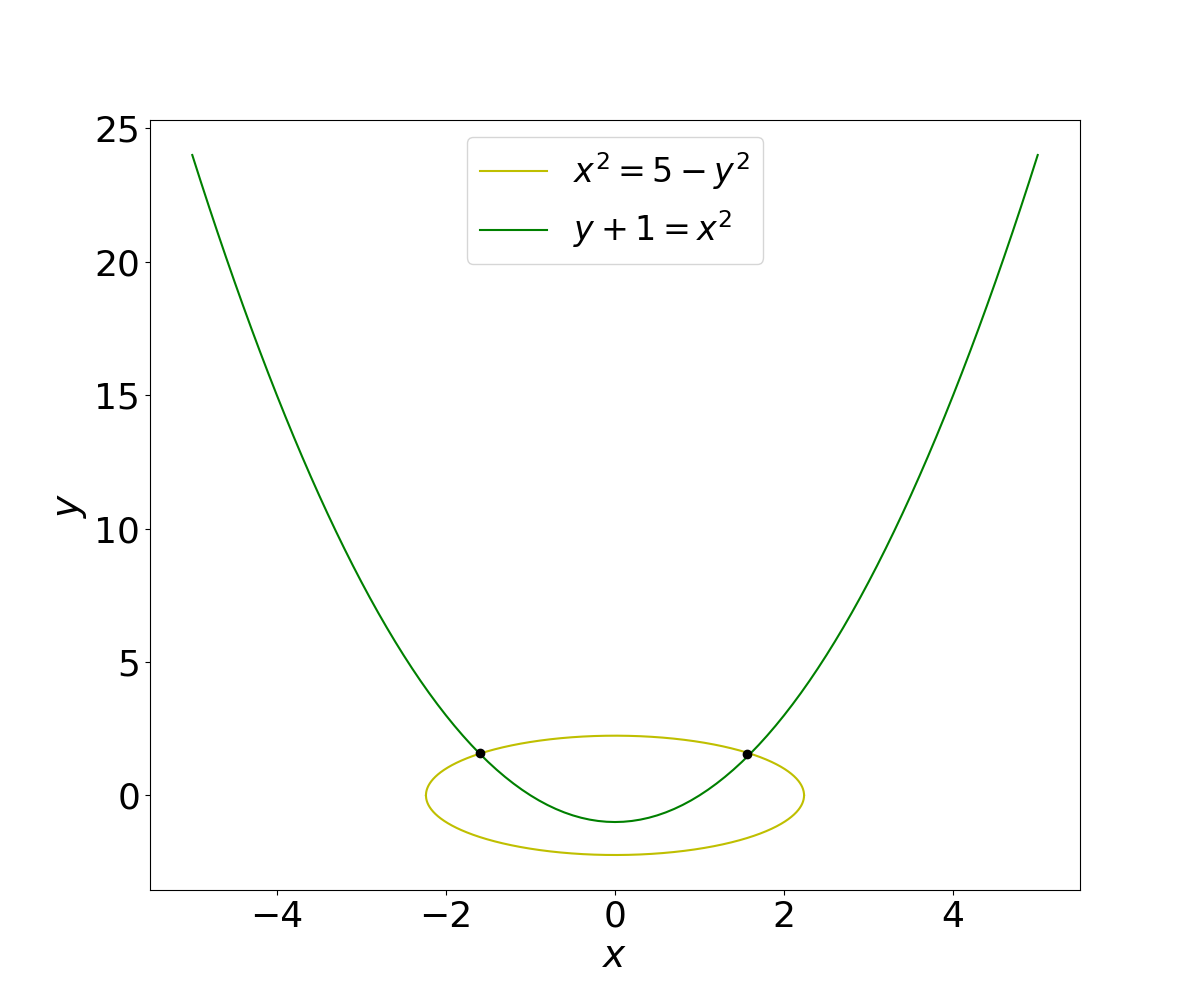
\includegraphics[width=\columnwidth]{graficosistema2.png}
  \caption{Trajetórias das curvas parametrizadas $x^2=5-y^2$ e $y+1=x^2$ com destaque para os seus pontos de interseção (a preto) nas coordenadas $(x,y)=(1.60049,1.56155)$ e $(x,y)=(-1.60049,1.56155)$,}
  \label{graficosistema2}
\end{figure}
Podemos ver como as duas curvas se intercetam em $(x,y)=(1.60049,1.56155)$ e $(x,y)=(-1.60049,1.56155)$, que, desta forma, são as soluções reais do sistema (2).\\
Definamos agora a função\\
\begin{minipage}[hbt!]{0.45\columnwidth}
$$f(x,y)=
\begin{bmatrix}
  x^2 + y^2 - 5\\
  -x^2 + y + 1
\end{bmatrix}
$$
\end{minipage}
e
\begin{minipage}[hbt!]{0.45\columnwidth}
$$J(x,y)=
\begin{bmatrix}
  2x & 2y\\
  -2x & 1
\end{bmatrix}
$$
\end{minipage}\\
em que $J(x,y)$ é a matriz jacobiana de $f$. De seguida aplicamos o método de Newton para encontrar os mínimos de $f$, que serão também as soluções do sistema (2), com uma precisão de $10^{-6}$ e um máximo de $100$ iterações. O método de Newton implica a resolução do sistema linear $Jd_k=f$, em que $d_k$ é o salto a ser dado na direção do eixo $0k$. Para resolver este sistema linear recorreu-se ao método de eliminação de Gauss com escolha parcial de pivot. Na Figura 3 encontra-se representada a trajetória seguida pelo método de Newton para encontrar soluções do sistema (2), partindo de pontos iniciais diferentes.
\begin{figure}[hbt!]
  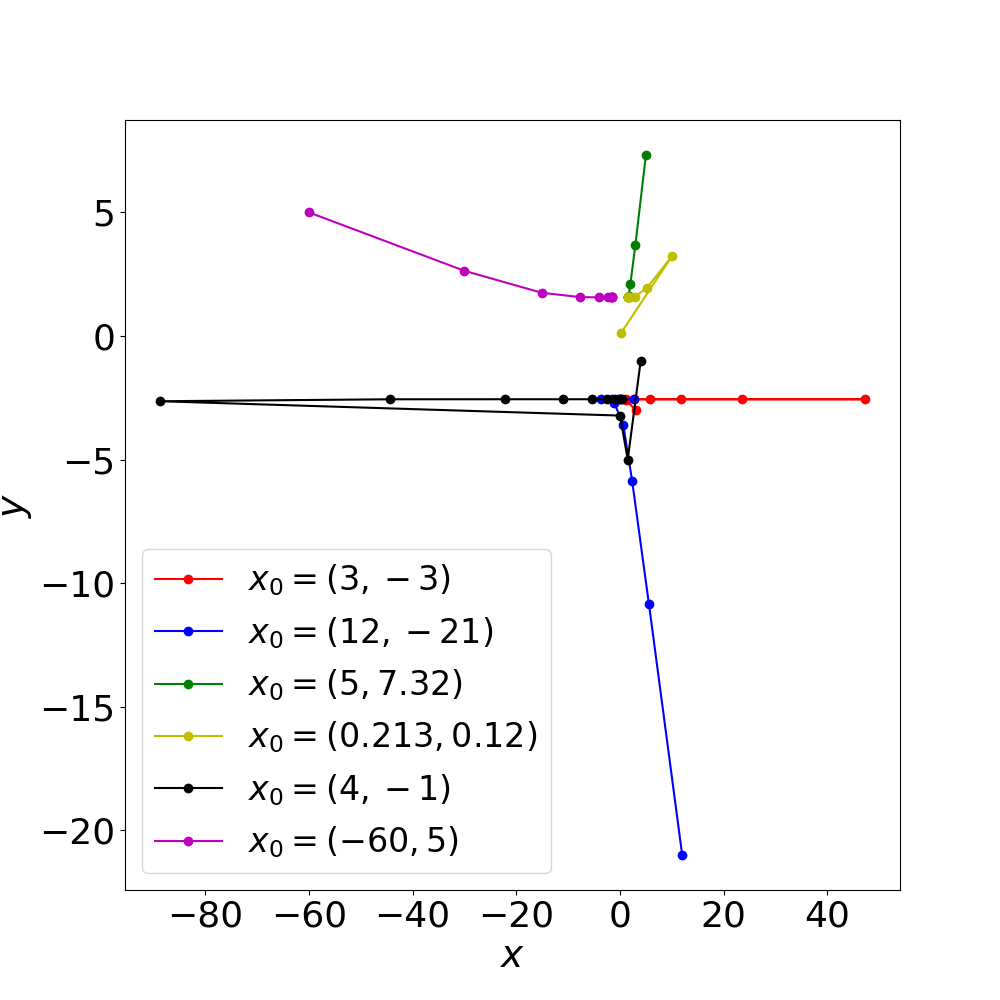
\includegraphics[width=\columnwidth]{nonlinearsystemtrajectorie.png}
  \caption{Trajetórias seguidas pelo método de Newton para a resolução do sistema $x^2=5-y^2 \wedge y+1=x^2$ partindo de pontos iniciais diferentes.}
  \label{graficosistema2}
\end{figure}
Veja-se como nenhuns dos caminhos seguidos passam pela reta $y=0$. Para pontos iniciais escolhidos em $y<0$ os pontos convergem para ${(x,y)\in \mathbb{R}: 1.6<x<2.7, y=1.5615528128}$. Já para pontos iniciais escolhidos em $y>0$ os pontos convergem para ${(x,y)\in \mathbb{R}: 1.6<x<2.7, y=-2.5615528128}$. Veja-se como para pontos bastante distantes destas "zonas de soluções" temos saltos maiores do que na vizinhança destas, deve-se à derivadas direcionais maiores nessas zonas mais distantes que fazem com que o salto $d_k$ seja maior. Um caso interessante é o do caminho que parte de $(4,-1)$ (a preto), que aproxima-se inicialmente da zona de soluções e depois afasta-se para $x\approx-80$, no entanto já tendo encontrado o valor de $y$ da solução, convergindo para o $x$ da solução nas próximas7 iterações. Isto pode ser justificado por uma derivada parcial $df/dx$ muito alta o que fez com que o caminho se afasta-se tanto para a esquerda.

\pagebreak
\section{Máximo de um potencial}
Consideremos agora a função $U(x,y)=e^{-(x-5)^2-(y-5)^2}.$
Pretendemos encontrar o máximo de $U$ pelo método de Newton.
Na Figura 4 encontra-se o gráfico de $U(x,y)$.
\begin{figure}[hbt!]
  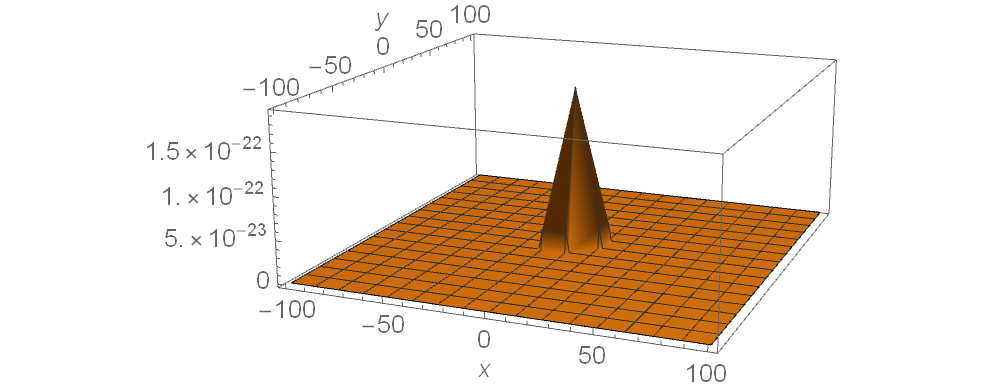
\includegraphics[width=\columnwidth]{potencial3D.png}
  \caption{Gráfico da função $U(x,y)$ em $-100<x<100$ e $-100<y<100$}
  \label{graficosistema2}
\end{figure}
Atendendo à Figura 4, vemos que o máximo está em $(0,0)$ e que a função é simétrica em relação à reta $y=-x$. Tendo isto em conta,
se nos restringirmos a encontrar o máximo de $U\restrict{y=-x}$, encontramos também o máximo de $U$.
Assim, substituindo em $U(x,y)$, o nosso problema resume-se a encontrar zeros de $U(x)=e^{-2x^2-50}$.
Para tal vamos aplicar o método de Newton à função $\frac{dU}{dx}=-4xe^{-2x^2-50}$, com precisão $10^{-6}$ e um número máximo de iterações $k_{max}=150$. Sabendo que o zero da função é em $x=0$, partimos de um ponto inicial próximo a este. Por exemplo $x_0=0.2$. Neste caso, a raíz de $\frac{dU}{dx}$ encontrada é $x=-4.4021166106886916\times10^{-11}$, e portanto é o máximo de $U(x)$ encontrado pelo método de Newton.\\
Tendo em conta a nossa restrição a $y=-x$, o máximo encontrado para $u(x,y)$ corresponde a $(x,y)=(-4.4021166106886916\times10^{-11},4.4021166106886916\times10^{-11})$.
\end{document}
